\chapter{Anforderungsanalyse}
% 1 Seite
Erreger in Krankenhäusern spielen eine immer größere Rolle, da mittlerweile Multiresistente Keime in Krankenhäusern existieren und Menschen mit hoch ansteckenden Krankheiten behandelt werden. Nach jeder Operation und jedem chirurgischen Eingriff sind medizinische Instrumente potentiell mit Keimen kontaminiert. Die Sterilisation, also die Entfernung von Keimen jeder Art ist Aufgabe der Zentralen Serilgutversorgung. 
\todo{...}
%
% - - - - - - - - - - - - - - - - - - - - - - - - 
%
\section{Ablauf der Medizinprodukteaufbereitung}
% 2 Seiten
Sterile chirurgische Instrumente werden in verschiedenen Abteilungen von Krankenhäusern und Kliniken verwendet. Sterile Instrumente werden in sterilen Verpackungen und -Containern transportiert und bis zu ihrem Einsatz steril gehalten. Bei ihrem Einsatz werden die Instrumente verschmutzt und potentiell kontaminiert. Sie werden anschließend gesammelt und zur ZSVA geliefert \cite[S.~7]{Ruther2014}.

Kontaminierte chirurgische Instrumente werden zum unreinen Bereich der ZSVA transportiert. Die Instrumente werden häufig mit Zusatzinformationen zu ihrem Zustand geliefert. Ein Angestellter der ZSVA ordnet die Instrumente nach Kategorien in Container ein. Die Zuordnung geschieht mittels Barcodes, die an den Instrumenten befestigt sind \cite[S.~9]{Ruther2014}.

Im anschließenden Reinigungsverfahren werden die Instrumente aus ihren Containern entfernt und meist in Reinigungsmaschinen gegeben. Manche Instrumente müssen jedoch von Hand gereinigt werden. Bei der Reinigung soll der Kontakt zwischen Mitarbeiter und Sterilgut so gering wie möglich gehalten werden. 

Nach der Reinigung wird das Sterilgut desinfiziert. Zu einer sichereren Desinfektion müssen die Geräte korrekt in Gitter einsortiert werden. Dabei hat jedes Instrument spezifische Eigenschaften, die beachtet werden müssen \cite[S.~11]{Ruther2014}.

Nachdem das Sterilgut desinfiziert wurde, wird es in den Sterilbereich der ZSVA überführt. Von nun an gilt es als Steril. Hier werden die Instrumente nochmals auf äußere Einflüsse hin untersucht. Spezielle Wünsche des Kunden, wie der Ersatz bestimmter Komponenten wird nun berücksichtigt. Es werden anschließend Beschriftungen an den Sterilgütern befestigt, die mittels eines Barcode-Lesers ausgelesen werden können.
Die Beschriftungen enthalten neben dem Barcode den Namen des Instruments oder Container und das Ablaufdatum, an dem die Sterilität abläuft. Das Sterilgut wird anschließend so verpackt, dass die Instrumente und Container bis zu ihrem Einsatz steril bleiben. Für jedes chirurgische Instrument gibt es eine charakteristische Anleitung, wie das Sterilgut zu verpacken ist.

\begin{figure}[htbp]
    \centering
    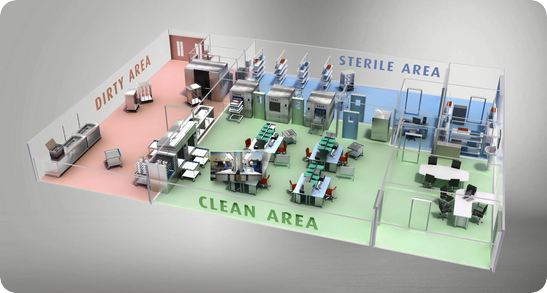
\includegraphics[width=1\textwidth]{data/bilder/clean-area-sterile-area.png}
    \caption{Schematischer Aufbau der Sterilgutversorgung \cite{Ives2017}}
    \label{fig:AufbauDerSterilgutversorgung}
\end{figure}

Wie in Abbildung \ref{fig:AufbauDerSterilgutversorgung} schematisch gezeigt, besteht die ZSVA aus drei Abschnitten: einer kontaminierten und unsauberen, einer sauberen und einer sterilen Abteilung. Diese drei Bereiche sind durch Desinfektions- und Sterilisationsmaschinen getrennt. Diese bilden eine Hygiene-Barriere zwischen den verschiedenen Hygieneleveln. Zwischen den unreinen- und reinen Bereichen bestehen Durchreichen, um Instrumente zwischen den Bereichen zurückreichen zu können, falls diese nicht korrekt gereinigt und desinfiziert wurden. \cite[S.~24]{Ruther2014}. Sterilgut kann nach der Behandlung in den Maschinen sehr heiß sein, was dazu führt, dass Mitarbeiter der Sterilgutversorgung strenge Sicherheitsvorkehrungen einhalten müssen sowie spezielle Kleidung tragen müssen. Dies ist besonders in der unreinen Abteilung nötig, da ebenfalls verhindert werden muss, dass sich Mitarbeiter mit Infektionen anstecken. Medizinische Instrumente sind mit Barcodes ausgestattet, welche in verschiedenen Schritten des Arbeitsprozesses ausgelesen werden. Computer sind essentieller Bestandteil der ZSVA, insbesondere der Reinabteilung. Hier unterstützen Softwarelösungen Mitarbeiter bei der Zusammenstellung der Instrumente. \cite[S.~25]{Ruther2014}.
%
% - - - - - - - - - - - - - - - - - - - - - - - - 
%
\section{Anforderungen bei der Medizinprodukteaufbereitung}
% 3 Seiten
In der Medizinprodukteaufbereitung werden mehrere tausend verschiedene medizinische Instrumente aufbereitet. Diese können sehr einfach bis sehr komplex strukturiert sein. Angestellte stehen oft unter hohem Zeitdruck und sind vielen Sicherheits- Hygienebestimmungen ausgesetzt. Es gibt zudem viele Fehlerquellen bei der korrekten Durchführung von Anweisungen, da Angestellte nicht immer alle Anweisungen und Anleitungen zu allen verschiedenen Instrumenten und allen einzelnen Prozesschritten kennen können.

In den heutigen ZSVAs finden sich typischerweise Barcodescanner für die automatische Prozessdokumentation. Instrumente werden in einem Behälter mit einem eindeutigen Identifizierungsetikett (Barcode) gesammelt. Für jeden Prozessschritt wird der Barcode gescannt und der Prozessschritt automatisch dokumentiert.

Angestellte im unreinen Bereich könnten von einem Assistenzsystem profitieren. 
In diesem Umfeld, in dem Oberflächen verschmutzt und kontaminiert sind, müssen spezielle hygienische Anforderungen erfüllt werden. So muss Sicherheitskleidung getragen werden. Klassische Desktop-Computer sowie Touchscreens sind hier aus hygienischen Gründen nicht einsetzbar.  \cite[S.~28]{Ruther2014}. Ein Assistenzsystem muss zudem abwaschbar sein und steril gehalten werden können. Es muss also möglich sein, die Hardware im unreinen Bereich anzuwenden. 

Eine wichtige Anforderung an Assistenzsysteme ist zudem die Akzeptanz durch die Anwender. So spielt die Benutzerfreundlichkeit des Systems eine wichtige Rolle. Das System sollte den regulären Workflow der Angestellten weder verzögern noch stören. Informationen müssen präzise und Kontextabhängig angezeigt werden. So muss der Angestellte selbst entscheiden können, zu welchem Instrument Zusatzinformationen angezeigt werden, da viele Instrumente und deren Behandlung wohl bekannt sind. Für diese Instrumente werden keine Zusatzinformationen benötigt und das System sollte keine Rolle spielen. Für unbekanntere und komplexere Instrumente müssen jedoch schnell Informationen angezeigt werden können, damit der Arbeitnehmer unterstützt werden kann. \cite[S.~29]{Ruther2014}


\todo{...}
%
% - - - - - - - - - - - - - - - - - - - - - - - - 
%
\section{Smartglasses im Bereich der Medizinprodukteaufbereitung}
% 1 Seite
\todo{...}
%
% - - - - - - - - - - - - - - - - - - - - - - - - 
%
\subsection{Einsatzmöglichkeiten}
% 4 Seiten
Heute müssen Angestellte der ZSVA zur Arbeit mit IT-Systemen an stationären Arbeitsplätzen arbeiten. Mobile Geräte wie Tablets erfordern eine Bedienung mit den Händen. Smartglasses dagegen sind immer einsatzbereit und ermöglichen völlig freihändiges Arbeiten. Sie ermöglichen den permanenten Zugriff auf Informationen und können so auch außerhalb des regulären Arbeitsplatzes eingesetzt werden. So können Angestellte der ZSVA auch beidhändig arbeiten. Beidhändiges Arbeiten ist in der ZSVA von großer Bedeutung.

Mithilfe der eingebauten Foto- und Videokamera können Arbeitsschritte lückenlos aufgezeichnet und dokumentiert werden. So können defekte oder problembehaftete Instrumente schnell dokumentiert werden.

Mithilfe von Smartglasses können Anleitungs- und Hilfevideos erstellt und abgerufen werden. So können erfahrene Angestellte für ihre unerfahreneren Kollegen Videos anfertigen, die zu einer Unternehmensinternen Wissensdatenbank erweitert werden können. Schritt-für-Schritt- Anleitungen können überforderungen von Mitarbeitern entgegenwirken und so die Arbeitsqualität erhöhen.

Schritt-für-Schritt Anleitungen erhöhen zudem die Flexibilität von Mitarbeitern im Unternehmen, da diese so an verschiedenen Stellen der Medizinprodukteaufbereitung eingesetzt werden können und dank der Unterstützung der Datenbrille möglicherweise auf Schulungen verzichten können. Monotonen Tätigkeiten wird somit ebenfalls vorgebeugt, da Angestellte so in verschiedenen Bereichen der ZSVA eingesetzt werden.

Treten Probleme im Arbeitsalltag auf, können Smartglasses auch dazu genutzt werden, mithilfe der Videokamera mit anderen Kollegen zu kommunizieren. So kann einem Gesprächspartner per Video das betreffende Sterilgut gezeigt werden und so schnell eine Lösung gefunden werden.

Smartglasses können auch dazu eingesetzt werden, Angestellte vor Gefahren zu warnen. So können Fehler im Arbeitsalltag verhindert werden und Prozesse sicherer gestaltet werden.

Smartglasses bieten nicht nur den immer perfekt eingestellten Bildschirm, der unabhängig von der Körpergröße des Anwenders ist, sondern lassen sich auch individualisieren. So kann ein Mitarbeiter die Datenbrille nach seinem Kenntnisstand einstellen und individuell anpassen. So kann auf Qualifikation, Erfahrung und Computer-Affinität eingegangen werden.

Ein Lagersystem kann die Handlungen der Benutzer koordinieren und somit Nutzern mitteilen, in welchem Arbeitsschritt sich andere Mitarbeiter befinden. So können redundante Arbeitsschritte verhindert werden. 
\todo{...}
%
% - - - - - - - - - - - - - - - - - - - - - - - - 
%
\subsection{Spezifische Anforderungen an Smartglasses im Bereich der Medizinprodukteaufbereitung}
% 3 Seiten
Smartglasses im Bereich der medizinprodukteaufbereitung müssen viele spezielle Anforderungen erfüllen. Es müssen im Gegensatz zu klassischen Computern mit Maus und Tastatur bzw. Touch-gesteuerten Geräten wir Tablets neuartige Bedienkonzepte verwendet werden. So lassen sich Smartglasses mittels Sparch- und Gestensteuerung bedienen.

Es ist nötig, neuartige User-Interfacesysteme zu entwickeln, die es ermöglichen, alle nötigen Informationen auf einem kleinen Display wie dem einer Datenbrille darzustellen. 

Smartglasses, die von Angestellten der ZSVA verwendet werden, müssen abwaschbar und steril gehalten werden können. Nur so kann es möglich sein, diese einzusetzen. 

Smartglasses müssen aufgrund des ganztägigen Einsatzes zudem weitere Harwareanforderungen erfüllen. Sie müssen möglichst leicht sein, damit sie die Angestellten in ihrer Arbeit nicht beeinträchtigen. Der Bedienkomfort der Brille hat hier einen großen Stellenwert. Zudem müssen sie einen ausreichend starken Akku haben, um 8 Stunden durchzuhalten bzw. müssen einen austauschbaren Akku haben.

Aufgrund der großen Lautstärke im Bereich der ZSVA muss die Sprachsteuerung in der Lage sein, auch bei großen Hintergrundgeräuschen die Sprachsteuerung gewährleisten zu können. Ebenfalls sollte die Sprachsteuerung auf eine Person abgestimmt werden können, damit mehrere parallel sprechende Menschen sich nicht gegenseitig beeinträchtigen.

\begin{comment}
Für den Einsatz von Smartglasses als allgegenwärtiges Informations- und Steuerungssystem für jeden einzelne(n) Mitarbeiter(in), ist die Verfügbarkeit aller erforderlichen Informationen aus allen relevanten Einzelsystemen in der ZSVA eine Grundvoraussetzung. Erst die semantische Vernetzung der Informationen aus unterschiedlichen Systemen der ZSVA (Reinigungs- & Desinfektionsgeräte, Sterilisatoren, Lagersysteme, Instrumentenmanagement-Software etc.) ermöglicht eine ganzheitliche Unterstützung der Mitarbeiter(innen) in allen Arbeitsschritten und somit die Reduzierung der Abhängigkeit von der Erfahrung, Qualifikation und Tagesform des/der einzelnen Mitarbeiters/-in, was wiederum zu einer signifikante Verbesserung der Qualität und Effizienz von Prozessen beiträgt (Ver- meidung von Fehlern, größere Reproduzierbarkeit).
\end{comment}
\todo{...}


%
% - - - - - - - - - - - - - - - - - - - - - - - - 
%
\subsection{Datenschutz}
% 0,5 Seiten
Der Einsatz von Smartglasses wird in der Literatur in Datenschutzrechtlicher Hinsicht diskutiert \cite{Berkemeier2017}. Smartglasses stellen eine nicht zu ignorierende Einschränkung in das Grundrecht auf informationelle Selbstbestimmung dar und erfordern damit völlig neue Anforderungen des Datenschutzrechts.

Besonderheit beim Einsatz von Smartglasses ist, dass diese im Betrieblichen Einsatz durchgängig genutzt werden und somit nicht nur die Nutzer der Brille, sondern auch alle in ihrem Umfeld befindlichen Personen durch die Grundrechtseingriffe der Brille betroffen sind. Aus Sicht des Datenschutzes sind Smartglasses den invasiven Technologien und Werkzeugen zu zuordnen \cite{Berkemeier2017}. Somit muss der Datenschutzaspekt essenzieller Bestandteil beim Design informationstechnischer Systeme in Smartglasses sein. 

Der rechtliche Rahmen für den Einsatz von Smartglasses in Unternehmen wird derzeit vom Bundesdatenschutzgesetz (BDSG), jedoch zunehmend auch durch den europäischen Rechtsrahmen gesetzt. Die im Mai 2017 in Kraft getretene EU-Datenschutzgrundverordnung (DSGVO) bildet den allgemeinen Rahmen der Datenschutzleitlinien. Grundsätzlicher Nenner der Rechtsgrundlagen ist, dass die Datensouveränität und Privatsphäre der Betroffenen vor Technologien geschützt wird. So müssen Vorkehrungen getroffen werden, die Erhebung, Speicherung und Nutzung von Daten zu reglementieren.
Die DSGVO regelt die rechtskonforme automatisierte Datenverarbeitung, genauer die Erhebung, Verarbeitung und Nutzung, von personenbezogenen Daten \cite{Berkemeier2017}. Die DGSVO stellt dabei einen ausführlichen  Pflichtenkatalog für die Verarbeitung personenbezogener Daten auf. Der Umfang hängt dabei von der Intensität des Eingriffs ab. Es sollten also nur Daten eroben werden, die keiner der besonders geschützten Kategorien zuzuordnen sind und dies nur im Aussmaß, die keine dauerhafte Speicherung erfordert. Werden personenbezogene Daten durch ein Unternehmen gespeichert, so setzt dies immer eine explizite Einwilligung voraus, die zu dokumentieren ist.

Smartglasses nehmen potentiell dauerhaft Video- und Tonaufnahmen auf und ermöglichen es per Gesichtserkennung Personen im Umfeld des Nutzers zu identifizieren. 
\todo{Quelle Spracherkennung/\\Gesichtserkennung}
Es ist ebenfalls potentiell möglich, den Nutzer der Brille zu überwachen. Es muss also sichergestellt werden, dass diese personenbezogenen Daten nicht gespeichert werden.
\todo{...}
%
% - - - - - - - - - - - - - - - - - - - - - - - - 
%
\subsection{Arbeitssicherheit}
% 0,5 Seiten
%
% - - - - - - - - - - - - - - - - - - - - - - - - 
%
\subsection{Grenzen des Einsatzes von Smartglasses}
% 2 Seiten  